\section{Lattice Paths}
\subsection{Problem Description}
Starting in the top left corner of a $2 \times 2$ grid, and only being able to move to the right and down, there are exactly
routes to the bottom right corner.

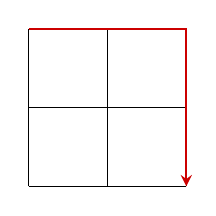
\begin{tikzpicture}
	\draw (0,0) grid (2, -2);
	\draw [->, >=stealth, thick, red!80!black] (0,0) -| (2, -2);
\end{tikzpicture}
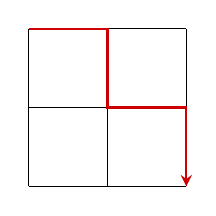
\begin{tikzpicture}
	\draw (0,0) grid (2, -2);
	\draw [->, >=stealth, thick, red!80!black] (0,0) -| (1, -1) -| (2, -2);
\end{tikzpicture}
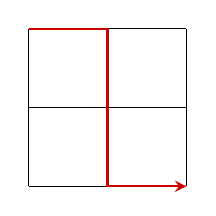
\begin{tikzpicture}
	\draw (0,0) grid (2, -2);
	\draw [->, >=stealth, thick, red!80!black] (0,0) -| (1, -2) -- (2, -2);
\end{tikzpicture}
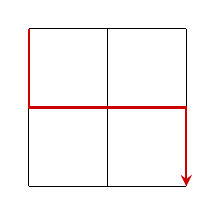
\begin{tikzpicture}
	\draw (0,0) grid (2, -2);
	\draw [->, >=stealth, thick, red!80!black] (0,0) |- (0, -1) -| (2, -2);
\end{tikzpicture}
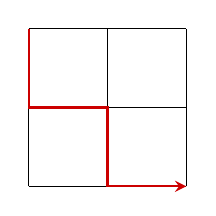
\begin{tikzpicture}
	\draw (0,0) grid (2, -2);
	\draw [->, >=stealth, thick, red!80!black] (0,0) |- (1, -1) |- (2, -2);
\end{tikzpicture}
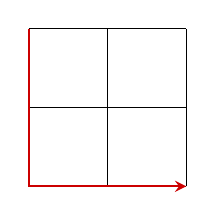
\begin{tikzpicture}
	\draw (0,0) grid (2, -2);
	\draw [->, >=stealth, thick, red!80!black] (0,0) |- (2, -2);
\end{tikzpicture}

How many such routes are there through a $20 \times 20$ grid?

\section{Solution}
\subsection{Combination}
\begin{align*}
	\binom nk = {}^nC_k & = \frac{n!}{(n-k)!k!}                              \\
						& = \frac{n \times (n - 1) \dots \times (k + 1)}{k \times (k - 1) \dots \times 1}
\end{align*}
